\documentclass[12pt]{article}
\usepackage[margin=2.5cm]{geometry}
\usepackage{enumerate}
\usepackage{amsfonts}
\usepackage{amsmath}
\usepackage{fancyhdr}
\usepackage{amsmath}
\usepackage{amssymb}
\usepackage{amsthm}
\usepackage{mdframed}
\usepackage{graphicx}
\usepackage{subcaption}
\usepackage{adjustbox}
\usepackage{listings}
\usepackage{xcolor}
\usepackage{booktabs}
\usepackage[utf]{kotex}
\usepackage{hyperref}

\definecolor{codegreen}{rgb}{0,0.6,0}
\definecolor{codegray}{rgb}{0.5,0.5,0.5}
\definecolor{codepurple}{rgb}{0.58,0,0.82}
\definecolor{backcolour}{rgb}{0.95,0.95,0.92}

\lstdefinestyle{mystyle}{
    backgroundcolor=\color{backcolour},
    commentstyle=\color{codegreen},
    keywordstyle=\color{magenta},
    numberstyle=\tiny\color{codegray},
    stringstyle=\color{codepurple},
    basicstyle=\ttfamily\footnotesize,
    breakatwhitespace=false,
    breaklines=true,
    captionpos=b,
    keepspaces=true,
    numbers=left,
    numbersep=5pt,
    showspaces=false,
    showstringspaces=false,
    showtabs=false,
    tabsize=1
}

\lstset{style=mystyle}

\pagestyle{fancy}
\renewcommand{\headrulewidth}{0.4pt}
\lhead{Team Treehouse}
\rhead{Java Objects Part 4 Notes}

\begin{document}
\title{Java Objects Part 4 Notes}
\author{Team Treehouse}
\maketitle

\section{Exceptions}

\bigskip

\begin{center}
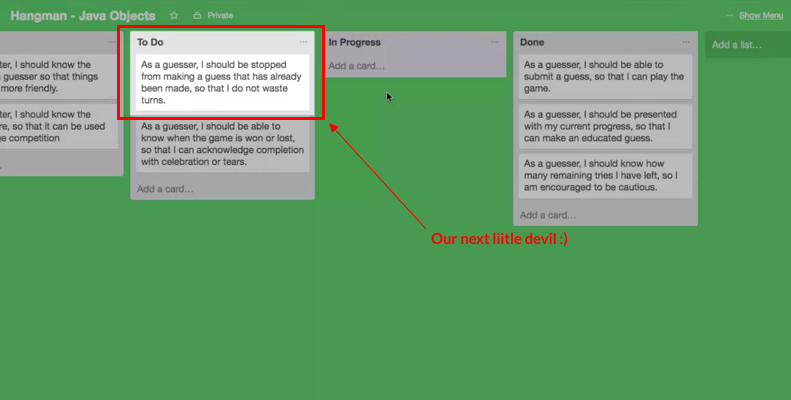
\includegraphics[width=\linewidth]{images/part_4_notes_1.png}
\end{center}

\begin{itemize}
    \item \textit{throw new EXCEPTION\_NAME:} raises exception \textit{EXCPETION\_NAME}
    \item \textit{try} and \textit{catch:} handles expections

    \begin{lstlisting}[language=Java,caption={lesson\_01/Game.java}]
    public class Game {
        ...
        public boolean applyGuess(char letter) {
            if (misses.indexOf(letter) != -1 || hits.indexOf(letter) != -1) {
                throw new IllegalArgumentException(letter + " has already been guessed"); // <- this little guy here :)
            }

            ...
        }

        ...
    }
    \end{lstlisting}

    \begin{lstlisting}[language=Java,caption={lesson\_01/Prompter.java}]
    import java.util.Scanner;

    public class Prompter {
        ...
        public boolean promptForGuess() {
            ...
            boolean isHit = false;
            try { // <- And this little guy here :)
                isHit = game.applyGuess(guess);
            } catch (IllegalArgumentException iae) {
                System.out.println(iae.getMessage());
            }

            return isHit;
        }
    }
    \end{lstlisting}

    \bigskip

    \underline{\textbf{Notes:}}

    \bigskip

    \begin{itemize}
        \item Files can be compiled and displayed by typing \textit{javac Example.java \&\& java Example}
        in terminal
    \end{itemize}
\end{itemize}

\bigskip

\section{Validating and Normalizing User Input}

\bigskip


\begin{center}
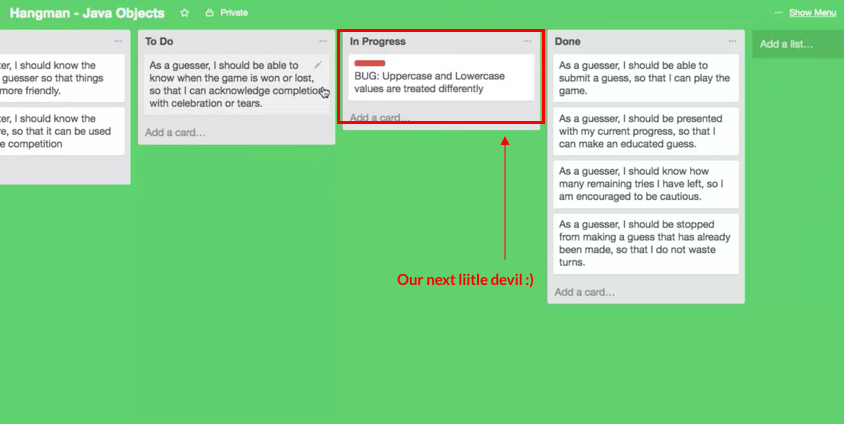
\includegraphics[width=\linewidth]{images/part_4_notes_2.png}
\end{center}

\begin{itemize}
    \item \textit{Character.toLowercase(CHAR\_VAR)}: turns value in \textit{CHAR\_VAR}
    to a lowercase character


    \begin{lstlisting}[language=Java,caption={lesson\_02/Game.java}]
    public class Game {
        ...
        private char normalizeGuess(char letter) {
            ...
            letter = Character.toLowercase(letter); // <- This little guy here :)
            ...
        }
    }
    \end{lstlisting}

    \bigskip

    \underline{\textbf{Notes:}}

    \bigskip

    \begin{itemize}
        \item Files can be compiled and displayed by typing \textit{javac Example.java \&\& java Example}
        in terminal
    \end{itemize}
\end{itemize}

\bigskip

\section{Exercise 2}

\bigskip

\begin{itemize}
    \item Solution included in \textit{exercise\_2.java}
\end{itemize}

\bigskip

\end{document}